\chapter{Methodik}

Nachfolgdend wird die vollständige Vorgehensweise der Versuchsdurchführung erklärt.
Dazu ist es notwendig eine Methodik zu definieren.

In der Browserforensik ist eine definierte Methodik notwendig, um die Komplexität moderner Browser zu bewältigen. Sie bildet bildet eine wissenschaftliche Basis für den durchgeführten Versuch sowie einen Leitfaden für Ermittler bei zukünftigen Untersuchungen. \cite{Aggarwal.2010, Izzati.2022, Horsman.2019}	
Ein oft verwendetes Vorgehensmodell in der Computer Forensik ist das "Generic Model Computer Forensics Investigations", kurz GCFIM. \cite{Yusoff.2011}
Ähnlich zum "abschnittsbasierter Verlauf einer forensischen Untersuchung" des Bundesamt für Sicherheit in der Informationstechnik ist es in Phasen mit definierten Abläufen gegliedert.
% https://www.bsi.bund.de/SharedDocs/Downloads/DE/BSI/Cyber-Sicherheit/Themen/Leitfaden_IT-Forensik.pdf?__blob=publicationFile&v=2

Izzati et al. haben diese Phasen auf Browserforensik abgebildet: \cite{Izzati.2022}
\begin{itemize}
	\item Vorbereitung: Versuchsplanung und Konfiguration der Versuchsumgebung.
	\item Datensammlung: Speicherabbilder identifizieren und während des Browsing Szenarios erstellen. 
	\item Datenanalyse: Suche nach Browsing Artefakten in gesammelten Daten.
	\item Dokumentation: Vorgehensweise und gefundene Artefakte dokumentieren.
\end{itemize}

Die Dokumentationsphase entspricht in dieser Arbeit Kapitel "Vergleich der Browser" (TODO!). Die Methodik der anderen Phasen wird nachfolgend beschrieben.

\section{Vorbereitung}

In der Vorbereitungsphase wird der durchgeführte Versuch geplant sowie die Versuchsumgebung konfiguriert. \cite{Izzati.2022} Versuchsplanung zählt die Auswahl von Browsern und Tools sowie die Definition eines durchzuführenden Browsing-Szenarios. Die Konfiguration der Versuchsumgebung umfasst die Installation und Konfiguration der notwendigen Software und Hardware.

\subsection{Browserauswahl}

Für diese Arbeit dazu entschieden: zwei weit verbreitete Brower verwenden + zwei Browser mit verstärkem Schutz der Privatsphäre.

Laut Statistik "Global market share held by leading internet browsers from January 2012 to May 2023" (Stand 23. Mai 2023) von Statista ist Chrome mit 62,82\% der meistgenutzte Browser weltweit.
Danach folgen Safari (20,86\%), Edge (5,28\%) und Firefox (2,77\%). 
\begin{figure}[h!]
	\resizebox{\linewidth}{!}{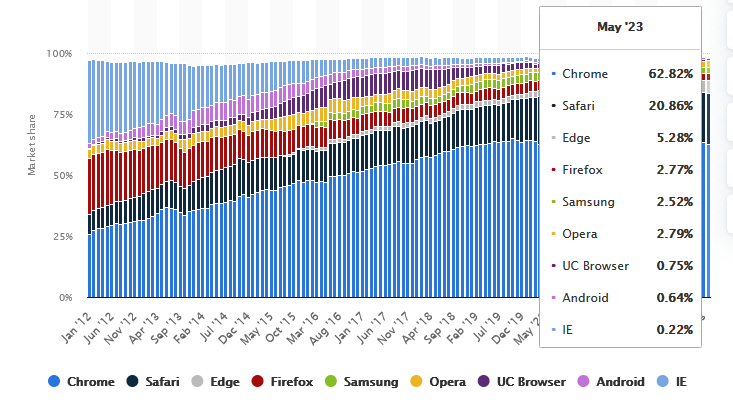
\includegraphics{bilder/browser-marketshare.png}}
%	\label{...}
	\caption{Tabelle mit wiederherstellbaren Dateien: Logfile 1 vs. Logfile 2}
\end{figure}

Problem: Safari hauptsächlich auf Mac OS genutzt, für Windows nur Safari 5.1.7 oder ältere Versionen.
Weiteres Problem: In Literatur zwar oft Internet Explorer (TODO: Quellen) untersucht, den Nachfolger Edge wurde bisher jedoch kaum in Literatur betrachtet.
	-> Nur 3 von 23 untersuchten Papern nahmen Edge mit in die Lister der analysierten Browser auf: \cite{Fayyad.2021, Horsman.2019, Gabet.2018}
	-> Ziel der Arbeit: keine neuen wissenschaftlichen Erkenntnisse.

Deshalb: wird neben Chrome noch Firefox als zweiter "regulärer" Browser aufgenommen:
Sowohl Firefox als auch Chrome werden in 15 von 23 untersuchten Papern analysiert: \cite{Aggarwal.2010, Oh.2011, Said.2011, Ohana.2013, Satvat.2014, Montasari.2015, Nalawade.2016, Rochmadi.2017, Gabet.2018, Md.2018, Muir.2019, Horsman.2019, Mahlous.2020, Fayyad.2021, Izzati.2022}

Weiterhin werden zwei Browser mit verstärkem Schutz der Privatsphäre ausgewählt.
Um die Browser mit den regulären Browsern vergleichen zu können, werden Browser gewählt, die auf den regulären Browsern basieren.
Basierend auf Chromium wird der Browser "Brave" gewählt.
Für Firefox wird der Tor-Browser gewählt, eine modifizierte Version von Firefox.

\subsubsection*{Firefox}

Der Browser Mozilla Firefox, kurz Firefox, ist ein open-source Webbrowser der gemeinnützigen Organisation Mozilla. 
Seit seiner Einführung im Jahr 2004 hat sich Firefox als beliebter Webbrowser etabliert. 

Mozilla bewirbt den Firefox Browser mit seinem Fokus Privatsphäre und Sicherheit.
Im Jahr 2009 führte Firefox den "privaten Modus" ein, der es Benutzern ermöglichte, das Surfen im Internet ohne Speicherung von Verlaufsdaten und Cookies zu genießen.
Abbildung X und Y (TODO!) zeigen, die Aktivierung des privaten Modus über das Menü in der rechten oberen Fensterecke. Der private Modus öffnet sich anschließend in einem neuen Firefox-Fenster

\begin{figure}[h!]
	\resizebox{\linewidth}{!}{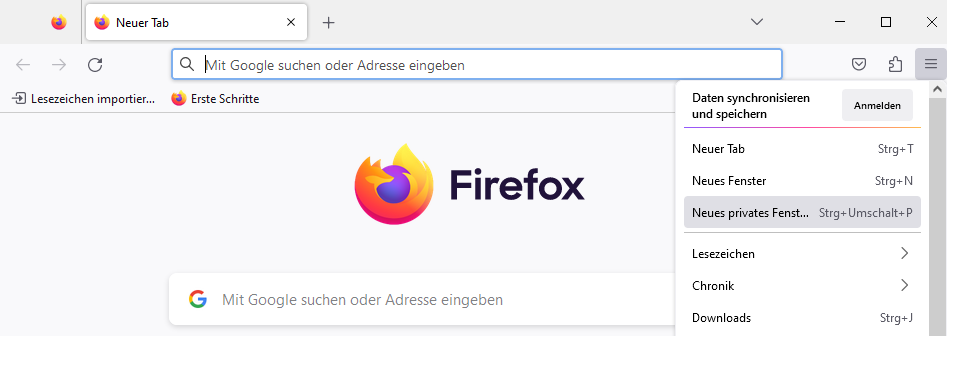
\includegraphics{bilder/firefox-private-mode.png}}
%	\label{...}
	\caption{Private Mode Firefox 1}
\end{figure}

\begin{figure}[h!]
	\resizebox{\linewidth}{!}{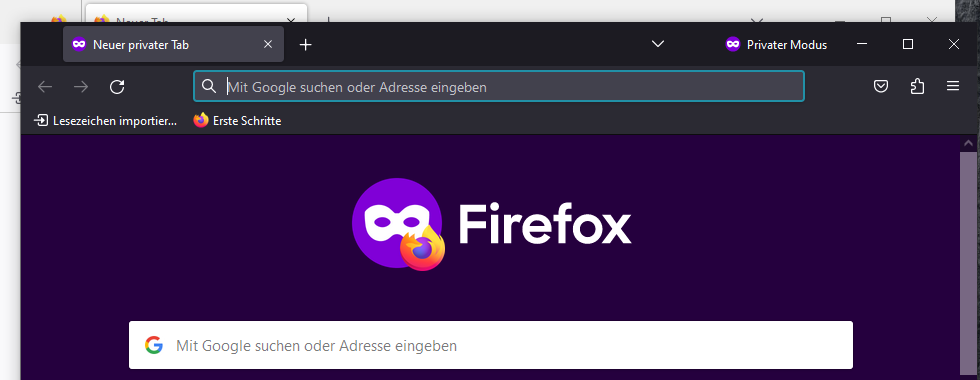
\includegraphics{bilder/firefox-private-mode2.png}}
%	\label{...}
	\caption{Private Mode Firefox 2}
\end{figure}

- Mozilla garantiert über den privaten Modus, dass Surfaktivitäten vor anderen Personen verborgen werden, die Firefox am selben Computer wie Sie verwenden. 
- Dazu zählt laut Mozilla: Passwörter, Chronik und Cookies gespeichert werden.
Dies Entspricht dem Schutz gegenüber des "Lokalen Angreifers", wie er in Kapitel X (TODO!) definiert ist.
- Es wird ausdrücklich darauf hingewiesen, dass die besuchten Webseiten und Ihr Internetanbieter (ISP)  weiterhin anhand Ihrer IP-Adresse Informationen über die von Ihnen besuchten Seiten sammeln, selbst wenn Sie nicht angemeldet sind. 
% https://www.mozilla.org/de/firefox/
% https://www.mozilla.org/de/about/history/

Somit ist der private Modus von Firefox laut Mozilla vor dem lokalen Angreifer geschützt, jedoch nicht vor dem Webangreifer.

Für diesen Versuch: Firefox Version 112.0.2 (64 Bit)

\subsubsection*{Tor}

Der Tor Browser, früher Tor Browser Bundle, ist ein auf Firefox basierender Webbrowser, der das Tor-Netzwerk nutzt.
- wird von der gemeinnützigen Organisation "The Tor Project" entwickelt
- Das Tor-Netzwerk ist ein Netzwerk virtueller Tunnel, der den Datenverkehr über drei zufällige Server ("Relays") im Tor-Netzwerk leitet, bevor er über den letzten Server (Exit-Relay) ins öffentliche Internet gelangt.
- Jedes Relay kennt nur den vorherigen und den nächsten Schritt des Datenverkehrs, aber nicht den gesamten Pfad oder die Quelle der Verbindung.
- Dadurch soll Privatsphäre und Sicherheit im Internet geschützt und verbessert werden.
- Das Tor-Netzwerk wird von einer dezentralen Community von Freiwilligen betrieben und verwaltet
- Der Tor Browser ermöglicht es Benutzern, Domains mit .onion als Top-Level-Domain zu besuchen. Die Domainnamen werden kryptografisch generiert und lassen nicht auf den Webseitennamen schließen. 

Über Tor-Browser mit Tor-Netzwerk verbinden:
\begin{figure}[h!]
	\centerline{\resizebox{\linewidth}{!}{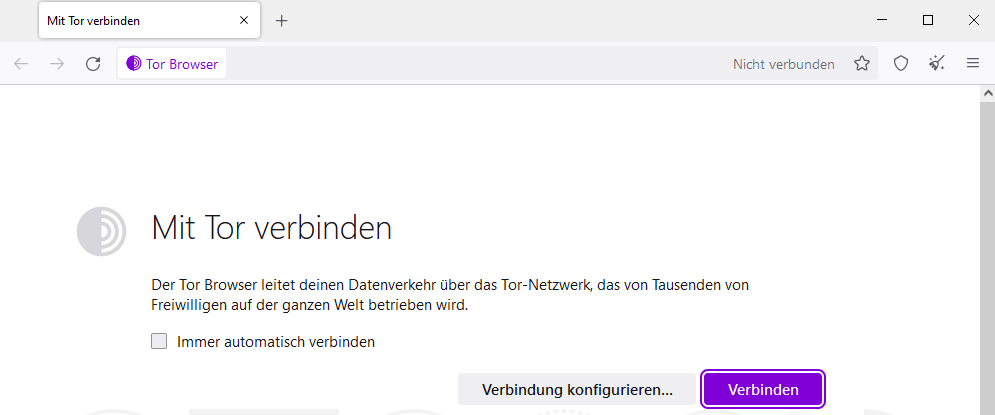
\includegraphics{bilder/tor-connect1.png}}}
%	\label{...}
	\caption{Tabelle mit wiederherstellbaren Dateien: Logfile 1 vs. Logfile 2}
\end{figure}
\begin{figure}[h!]
	\centerline{\resizebox{\linewidth}{!}{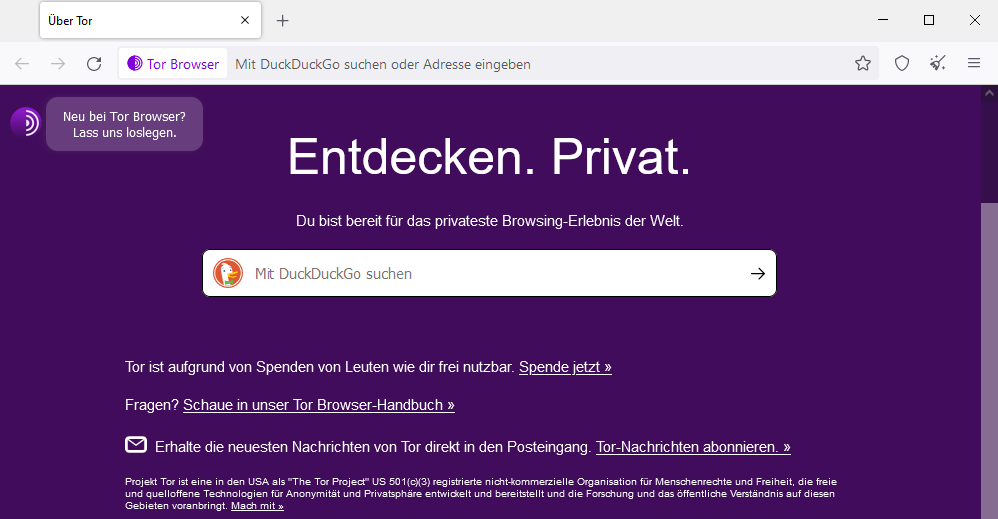
\includegraphics{bilder/tor-connect2.png}}}
%	\label{...}
	\caption{Tabelle mit wiederherstellbaren Dateien: Logfile 1 vs. Logfile 2}
\end{figure}

Der Tor Browser wirbt im Gegensatz zu Firefox mit folgendem Schutzmaßnahmen gegen Webangreifer:
- Internetdienstanbieter können Internetaktivitäten aufgrund Natur des Tor-Netzwerks nicht verfolgen 
- Die Betreiber der besuchten Websites sehen eine Verbindung vom Tor-Netzwerk anstelle der echten IP-Adresse des Rechners
- Kein "fingerprinting” = Nutzer anhand Browserkonfiguration identifizieren.

Der Tor Browser wirbt mit folgendem Schutzmaßnahmen gegen lokalen Angreifer:
- Schutz vor lokalem Angreifer durch Modifikation von Firefox: Tor Browser basiert auf dem Extended Support Release von Firefox.
- Lokaler Angreifer: Tor Browser does not keep any browsing history. Cookies are only valid for a single session (until Tor Browser is exited or a New Identity is requested).
- Technische Umsetzung
1. Standardeinstellungen geändert
2. Zusätzliche Erweiterungen installiert:
	- Torbutton": Mit Tor verbinden" -> Screenshot
	- "NoScript":  JavaScript und andere potenziell schädliche Inhalte nur von vertrauenswürdigen Websites Ihrer Wahl ausgeführt

Zusätzliche Funktion: "Neue Identität"
\begin{figure}[h!]
	\resizebox{\linewidth}{!}{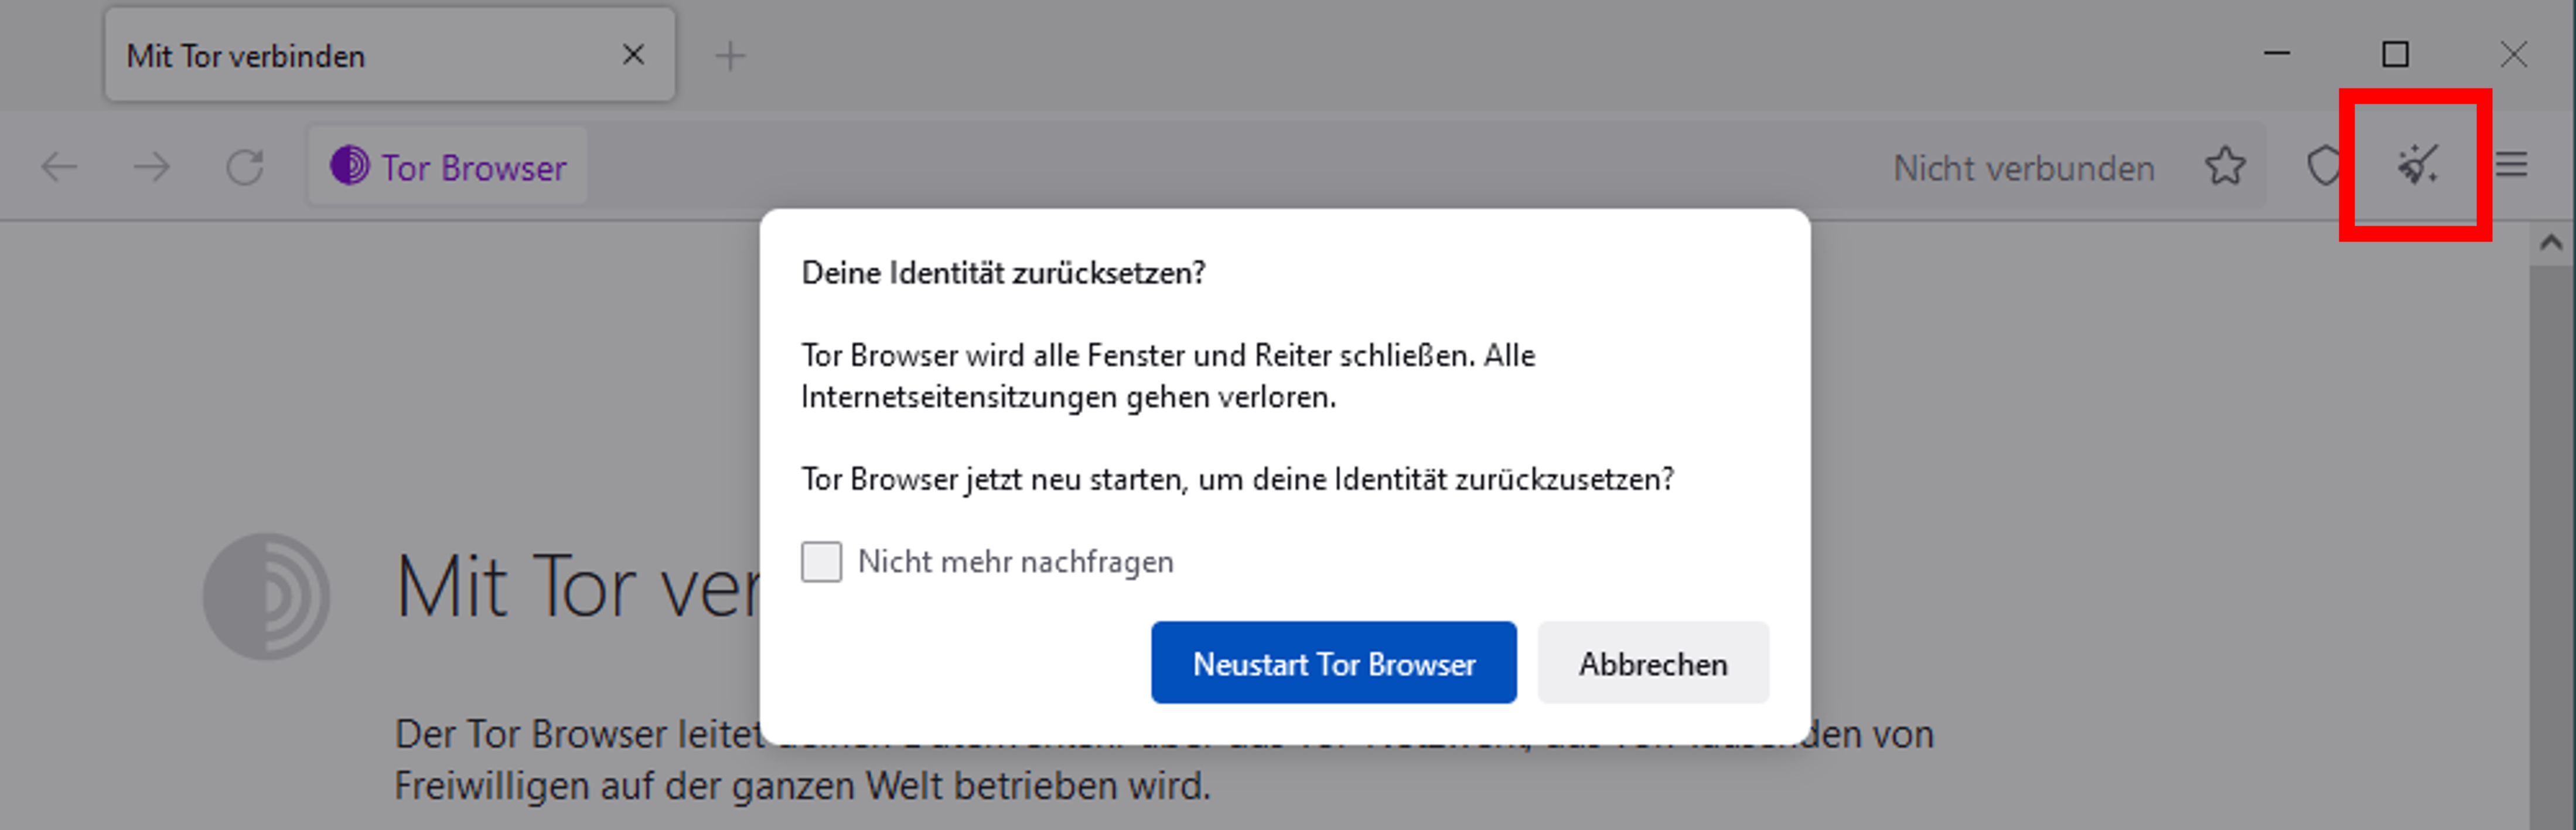
\includegraphics{bilder/tor-new-identity.png}}
%	\label{...}
	\caption{Tabelle mit wiederherstellbaren Dateien: Logfile 1 vs. Logfile 2}
\end{figure}
Die Funktion "Neue Identität" im Tor Browser ermöglicht es, alle aktuellen Tabs und Fenster zu schließen, sämtliche private Informationen wie Cookies und Verlauf zu löschen und für alle Verbindungen neue Relays zu verwenden.

Für diesen Versuch: Tor Version 12.0.4 (64 Bit)

\subsubsection*{Chrome}

\subsubsection*{Brave}

\subsection{Browsing Szenario}

Siehe Ziel der Arbeit: Versuch soll nicht Situation eines Ermittlers simulieren, der eine unbekannte Datenlage hat.
Stattdessen: Bereits vor Analyse bekannt, nach welchen Daten gesucht werden muss.

Deshalb wird für Versuch definiert, mit welchen Daten der Rechner kontaminiert werden soll.

Im Falle der Browser-Forensik wird dazu ein sog. "Browsing Szenario" festgelegt. (TODO: Quelle, alternative Namen).

Dabei handelt es sich um Reihe von fest definierten Aktivitäten, die für jeden zu untersuchenden Browser durchgeführt werden.

Anforderungen an Browsing Szenario 
- Ziel: PB Artefakte, die ausschließlich in Browsing-Szenario vorkommen, bspw. "twitter" oder "facebook" bereits in vielen Windows-Standardanwendungen enthalten.
- (TODO: Literatur)

Folgende Schritte werden in jedem Browser durchgeführt: 

\begin{enumerate}
\item  www.google.com aufrufen
	\begin{enumerate}[label*=\arabic*.]
	\item Alle Cookies akzeptieren 
	\item Google-Suche nach "pfaffenhofen"
	\end{enumerate}
\item www.google.com aufrufen
	\begin{enumerate}[label*=\arabic*.]
	\item Cookies alle akzeptieren 
	\item Google-Suche nach "nanoradar" 
	\end{enumerate}
\item www.google.com aufrufen
	\begin{enumerate}[label*=\arabic*.]
	\item Cookies alle akzeptieren 
	\item Google-Suche nach "mallofamerica"
	\item Auf Suchergebnis "mallofamerica.com" klicken
	\end{enumerate}
\item www.google.com aufrufen
	\begin{enumerate}[label*=\arabic*.]
	\item Cookies alle akzeptieren 
	\item Google-Suche nach "mooserliesl"
	\item Auf Suchergebnis "mooserliesl.de" klicken
	\end{enumerate}
\item "www.unitree.com" über URL-Leiste öffnen
\item "www.donaukurier.de" über URL-Leiste öffnen
	\begin{enumerate}[label*=\arabic*.]
	\item Donaukurier Logo in neuem Tab öffnen
	\end{enumerate}
\item "mail.google.com" über URL-Leiste öffnen
	\begin{enumerate}[label*=\arabic*.]
	\item Mit google Account anmelden: 
			\begin{enumerate}[label*=\arabic*.]
			\item E-Mail = "computerforensikvl@gmail.com"
			\item Passwort = "Vorlesung23!"
			\end{enumerate}
	\item Neue E-Mail schreiben:
			\begin{enumerate}[label*=\arabic*.]
			\item Empfänger: "cas0597@thi.de" und "chs3702@thi.de"
			\item Betreff: "Betrefftext"
			\item Mailinhalt: "Mailinhalt"
			\end{enumerate}			
	\end{enumerate}
\end{enumerate}

Aus diesem Browsing-Szenario lassen sich sogenannte "private Browsing Artefakte", kurz PB Artefakte ableiten.
Wie in Kapitel X (TODO!) beschrieben, handelt es sich dabei um Strings oder reguläre Ausdrücke, die eindeutig einem Schritt im Browsing-Szenario zugeordnet werden können.
PB Artefakte in Tabell X (TODO!) beschrieben.

Bemerkung: "mail.google.com" nicht aufgeführt, da festgestellt, dass URL bereits in vielen Windows Standardanwendungen enthalten ist.

\begin{table}[]
\begin{tabular}{|c|l|c|}
\hline
\textbf{Kategorie}           & \multicolumn{1}{c|}{\textbf{Private Browsing Artefakt}}                                      & \textbf{\begin{tabular}[c]{@{}c@{}}Schritt im\\  Browsing Szenario\end{tabular}} \\ \hline
\multirow{4}{*}{Suchbegriff} & "pfaffenhofen"                                                                               & 1.2                                                                              \\ \cline{2-3} 
                             & "nanoradar"                                                                                  & 2.2                                                                              \\ \cline{2-3} 
                             & "mallofamerica"                                                                              & 3.2                                                                              \\ \cline{2-3} 
                             & "mooserliesl"                                                                                & 4.2                                                                              \\ \hline
\multirow{4}{*}{URL}         & "mooserliesl.de"                                                                             & 3.3                                                                              \\ \cline{2-3} 
                             & "mallofamerica.com"                                                                          & 4.3                                                                              \\ \cline{2-3} 
                             & "unitree.com"                                                                                & 5.                                                                               \\ \cline{2-3} 
                             & "donaukurier.de"                                                                             & 6.                                                                               \\ \hline
Bild                         & \begin{tabular}[c]{@{}l@{}}0x89 0x50 0x4E 0x47 ...\\ (PNG als Hexadezimalwerte)\end{tabular} & 6.1                                                                              \\ \hline
\multirow{4}{*}{E-Mail}      & "computerforensikvl@gmail.com"                                                               & 7.1.1                                                                            \\ \cline{2-3} 
                             & "Vorlesung23!"                                                                               & 7.1.2                                                                            \\ \cline{2-3} 
                             & "cas0597@thi.de"                                                                             & 7.2.1                                                                            \\ \cline{2-3} 
                             & "chs3702@thi.de"                                                                             & 7.2.1                                                                            \\ \hline
\end{tabular}
\end{table}


\subsection*{VM Konfiguration}

Best Practice in Browser Forensik: Versuche sowie Analysen in virtualisierter Umgebung durchführen. (TODO: Quellen)
- Dadurch Reproduzierbarkeit der Ergebnisse sichergestellt
- Keine Vermischung der PB Artefakte, wenn gleicher Rechner verwendet
- Keine Vermischung der Versuchsumgebung mit der Analyseumgebung
- Ergebnisse sind transportabel -> Zustände von Virtuellen Maschinen exportierbar
- Deshalb oft in Literatur empfohlen

Als Virtualisierungssoftware für Versuch verwendet: Kostenlose Oracle VirtualBox VM, Version 7.0.8 r156879 (Qt5.15.2)

In Literatur zu Browserforensik empfohlen: pro Browser eine VM erstellen, auf der Browsing Szenario durchgeführt wird.

Daui zunächst eine Benchmark-VM erstellt. Wird nach Basiskonfiguration als OVA exportiert und für jeden Browser dupliziert. Anschließend für jede VM entsprechenden Browser installiert.

\paragraph*{Betriebssystem}
VM Betriebssystem: In den 23 untersuchten wissenschaftlichen Veröffentlichungen wurden die privaten Browsermodi ausschließlich unter Windows untersucht.
Da Ziel dieser Arbeit ist keine neuen wissenschaftlichen Ergebnisse: Für diesen Versuch Windows 10 verwendet.
Deshalb auf VM installiert: Windows 10 Pro, Build: 19045.2006, nicht aktiviert

\paragraph*{Speicher}
In Literatur keine Angaben über empfohlene Festplattengrößen.
Deshalb an Microsoft Empfehlungen orientiert: VM erhält 30 GB (VDI-Format) Festplatte, kein SSD-Laufwerk
% https://support.microsoft.com/en-us/windows/windows-10-system-requirements-6d4e9a79-66bf-7950-467c-795cf0386715
In Literatur ebenfalls kaum Angaben über empfohlene RAM Größe gemacht:
> Wichtige Entscheidung, da wie später in Kapitel X beschrieben, RAM-Größe Auswirkungen auf Ergebnisse hat
> Rochmadi et al.: 2 GB \cite{Rochmadi.2017}
> Ohana et al.: 4 GB \cite{Ohana.2013}: 
> Hier: mit 6 GB die maximal mit verfügbaren Speicherresourcen auf Analyserechner mögliche Größe gewählt, um später Speicherabbilder des Arbeitsspeichers zu sichern.

\paragraph*{Netzwerkkonfiguration}
VM wurde mittels Netzwerkbrücke direkt mit dem physischen Netzwerk des Hostsystems verbunden. Somit erhält jede virtuelle Maschine eine eigene IP-Adresse im Netzwerk des Rechners, auf dem die VM läuft.
Der Netzwerkadapter der VM wurde erst nach Browserinstallation aktiviert, um eine versehentliche Kontaminierung der VM zu vermeiden.

\subsubsection*{Installierte Programme auf VM}
Um Programme auf VM zu installieren: Gemeinsamer Order zwischen VM und Rechner eingerichtet, auf dem VM läuft. Ordner wird in VM als Netzwerklaufwerk angezeigt
Grund: VM erst mit Beginn von Browsing Szenario mit Netzwerk und Internet verbinden. Deshalb: Programme mussten auf Rechner auf dem VM läuft heruntergeladen werden und über gemeinsamen Order auf VM transportiert werden.

\paragraph*{Browserinstallation}
Zunächst Browser installiert. Folgende Installationsverzeichnisse verwendet:
\begin{enumerate}
\item[\textbf{Firefox}] \texttt{C:\\Program Files\\Mozilla Firefox\\firefox.exe}
\item[\textbf{Tor}] \texttt{C:\\Program Files\\Tor Browser\\Browser\\firefox.exe}
\item[\textbf{Chrome}] ***TODO!***
\item[\textbf{Brave}] ***TODO!***
\end{enumerate}

Weiterhin wurden zwei Werkzeuge der Sysinternal-Abteilung von Microsoft installiert: "Process Monitor" und "Process Explorer". 
Hintergrund: siehe Ziel der Arbeit: ersuch soll nicht Situation eines Ermittlers simulieren, der eine unbekannte Datenlage hat. Mithilfe der Tools soll Browserverhalten während des Szenarios aufgezeichnet und untersucht werden können.

\paragraph*{Process Monitor}
Process Monitor ermöglicht die Aufzeichnung aller Aktivitäten und Ereignisse, die auf einem Windows-System im Zusammenhang mit Prozessen, Dateisystemen, Registrierungseinträgen und Netzwerkverbindungen stattfinden. Die Aufzeichnung kann als "Process Monitor Logfile" (PML) exportiert werden. Die aufgezeichneten Aktivitäten können somit beliebig gefiltert werden, beispielsweise nach Prozessnamen oder Operation, die der Prozess durchgeführt hat. Die Möglichkeit zum Export als CSV-Datei ermöglicht eine umfassende Untersuchung mit weitern Programmen, wie Microsoft Excel.
% https://learn.microsoft.com/de-de/sysinternals/downloads/procmon
Für diesen Versuch verwendet: Version 3.93

\paragraph*{Process Explorer}
Weiterhin wurde "Process Explorer" installiert. Das Tool erweitert die Funktionen des Windows Task Managers und ermöglicht es, einen umfassenden Überblick über alle aktiven Prozesse und deren Eigenschaften zu erhalten. Beispielsweise können alle ausgeführten Windows Dienste mit ihren PIDs angezeigt werden.
% https://learn.microsoft.com/de-de/sysinternals/downloads/process-explorer
Für diesen Versuch verwendet: Version 17.04

\subsection{Analysewerkzeuge}

Neben Konfiguration der VM muss Analyseumgebung vorbereitet werden.
Dazu: Diverse Tools zur Analyse installieren

\subsubsection*{Autopsy}
Wie im nächsten Kapitel X (TODO!) beschrieben, müssen Festplattenabbilder untersucht werden.
Dazu wird in der Literatur das Tool "Autopsy" empfohlen.

Autopsy ist ein Open-Source-Digital-Forensik-Tool, das auf der Sleuthkit-Bibliothek basiert. 
Sleuthkit ist eine Sammlung von Open-Source-Tools für die forensische Analyse von Dateisystemen. Es bietet Funktionen zum Lesen, Analysieren und Wiederherstellen von Daten aus verschiedenen Dateisystemen. 
Autopsy baut auf der Funktionalität von Sleuthkit auf und bietet eine grafische Benutzeroberfläche für die forensische Analyse. 
Wurde hauptsächlich in Java geschrieben.
Es erweitert die Funktionalität von Sleuthkit, indem es zusätzliche Tools, Plug-Ins und Automatisierungsfunktionen bereitstellt, um den forensischen Untersuchungsprozess zu unterstützen.
 
Für diesen Versuch verwendet: Version 4.20.0

\subsubsection*{Volatility}
Neben der Analyse von Festplattenabbildern müssen gemäß Kapitel X Abbilder des Arbeitsspeichers unteruscht werden. Dazu wird das in der Literatur empfohlene Tool "Volatility" verwendet.
 
Das Volatility Memory Forensics Framework ist ein Open-Source-Tool, das für die forensische Analyse von Arbeitsspeicherabbildern verwendet wird. Es ist speziell darauf ausgerichtet, Informationen und Artefakte aus dem physischen oder virtuellen Arbeitsspeicher eines Computers zu extrahieren.

Geschrieben in Python, frei auf GitHub verfügbar:	
Version: Volatility3, Version 2.4.1 (aktuellster Release)

Für diesen Versuch verwendet: "Volatility3"
= vollständige Neuschreibung des Volatility Memory Forensics Frameworks, die im Jahr 2020 veröffentlicht wurde. Behebt technische und Performanceprobleme der vorherigen Version.

Oft beworbender Vorteil von Volatility3: kein "Profile" mehr notwendig. Volatility3 erstellt Symboltabellen für Windows-Speicherabbilder basierend auf dem Speicherabbild selbst.
Dabei handelt es sich um ein Konfigurationseinstellung, welche die Speicherstruktur und die Verhaltensweisen des Betriebssystems definiert.
	% https://volatility3.readthedocs.io/en/latest/vol2to3.html
	% https://www.volatilityfoundation.org/
	% https://github.com/volatilityfoundation/volatility3

Volatility basiert auf Plugins, welche spezifische Funktionen und Analysen für verschiedene Aspekte des Systems bereitstellen. Für diesen Versuch werden folgende Plugins verwendet. 
\begin{itemize}
\item pslist	
\item yarascan		
\item memmap	 	
\item filescan
\item svcscan
\end{itemize}
		
Genaue Beschreibung der PlugIns und deren Zusammenhang: Siehe Analysephase in Kapitel X (TODO!).

\subsection*{Übersicht verwendete Software}

Tabelle X listet zusammenfassend alle in diesem Versuch verwendeten Software-Programme, deren Zweck sowie Version auf.

Neben den Programmen zur Analyse der Speicherabbilder: diverse zusätzliche unterstützende Tools zur vollständigen Analyse benötigt, diese werden nicht genauer beschrieben.
- Nur in Tabelle aufgenommen

\begin{table}[]
\resizebox{\linewidth}{!}{
\begin{tabular}{|l|l|l|}
\hline
\multicolumn{1}{|c|}{\textbf{Software}} & \multicolumn{1}{c|}{\textbf{Zweck}}                                              & \multicolumn{1}{c|}{\textbf{Version}} \\ \hline
Oracle VirtualBox                       & Virtualisierung                                                                  & 7.0.8 r156879                         \\ \hline
Windows 10 Pro                          & VM Betriebssystem                                                                & Build: 19045.2006                     \\ \hline
Process Monitor                         & Aufzeichnung Prozessaktivitäten                                                  & 3.93                                  \\ \hline
Process Explorer                        & Darstellung der Eigenschaften aktueller Prozesse                                 & 17.04                                 \\ \hline
Autopsy                                 & Analyse Festplattenabbilder                                                      & 4.20.0                                \\ \hline
Volatiltiy                              & Analyse RAM-Abbilder                                                             & Volatility3 Version 2.4.1             \\ \hline
HxD                                     & Analyse Binärdateien in hexadezimaler und ASCII-Darstellung                      & 2.5.0.0                               \\ \hline
Notepad++                               & Analyse strukturierter Dateiformate, z.B. JSON, XML                              & 8.4.5                                 \\ \hline
Registry Explorer                       & Grafischer Oberfläche zur Untersuchung von Windows-Registry Hives                & 2.0.0.0                               \\ \hline
DB Browser for SQLite                   & Grafische Oberfläche zur Verwaltung und Untersuchung von SQLite-Datenbanken      & 3.12.2                                \\ \hline
sqldiff.exe                             & Befehlszeilen-Programm zur Anzeige von Unterschieden zwischen SQLite-Datenbanken & 3.42.0                                \\ \hline
ChromeCacheView                         & Einlesen von Chrome Cache-Dateien und visuelle Aufbereitung des Inhalts          & 2.46                                  \\ \hline
MZCacheView                             & Einlesen von Firefox Cache-Dateien und visuelle Aufbereitung des Inhalts         & 2.21                                  \\ \hline
FirefoxCache2                           & Erweitert MZCacheView, um Firefox "index"-Cachedatei zu analysieren              & Commit b50ab4f                        \\ \hline
dejsonlz4                               & Dekomprimierung von .jsonlz4-Dateien                                             & Commit c4305b8                        \\ \hline
\end{tabular}
}
\end{table}



\section{Datensammlung}

\cite{Izzati.2022}
In der Identifikations- und Sammelphase werden alle potenziellen Beweismittel identifiziert, gekennzeichnet und gesammelt, um sie in der nächsten Phase zu verwenden.
> Browsing Szenario durchfüren

Gesammelte Daten:
> Process Monitor Logfiles:
	- siehe Ziel der Arbeit: "White-Box"-Ansatz: Versuch wird nicht aus Sicht von Forensiker durchgeführt, der nur begrenzten Zugriff auf Beweismittel hat. 
	- Sondern: Ziel ist das Verhalten von privaten Browsing möglichst vollständig zu untersuchen, um so viele Artefakte wie möglich zu identifizieren.
	- Deshalb: von Fayyad-Kazan et al. vorgeschlagen \cite{Fayyad.2021} Aktivitäten während Browsing-Szenario aufzeichnen mit "Process Monitor".
		> Während Browsing Szenario Filechanges untersuchen: DaemonFS set to monitor all activity within local hard drive\cite{Ohana.2013}
	- Aufgezeichnet werden Aktivitäten in beispielsweise der Registry, im Dateisystem und Netzwerkaktivitäten.
	- Mit grafischer Oberfläche: Start, Stopp und Sicherung der Aufzeichnung als PML Datei (Process Monitor Logfile) -> Kann in CSV Umgewandelt werden
	- Danach: Präzise Filterung der Ergebnisse. Fokus hier nach Esmpfehlung von Autoren in \cite{Fayyad.2021}: Schreibaktivitäten auf Dateien und in Registry. 
		- Registry: \cite{Rochmadi.2017}
			•	Das Windows-Registrierungsverzeichnis enthält viele Informationen zur Nutzung des Computers, Benutzerkonfigurationen, Anwendungen und Hardwaregeräte
			•	Informationen im Registrierungsverzeichnis werden nach Ausführungsreihenfolge, Suchschlüsselwörtern, zuletzt aufgerufenen Ordnern, Anwendungsprotokollen und anderen Kategorien sortiert.
	*** TODO: Shared Folder ***

> Speicherabbilder:
	> Hauptaufgabe eines Computer-Forensik-Ermittlers: Erwerb und Analyse von Speicherabbildern von Computervorrichtungen. \cite{Hassan.2019}
    > Speicherabbild = statischer Schnappschuss der Daten auf sekundärem Speicher (HDD, SSD), angeschlossenen Speichergeräten (USB-Stick, externe Festplatte, Magnetband) oder RAM-Speicher (bei Live-Erfassung auf laufenden Systemen). \cite{Hassan.2019}
    > Speicherabbild ist Container für Daten, der individuelle Dateien oder das gesamte Laufwerk/Live-Speicherdateien in einer Image-Datei speichern kann. \cite{Hassan.2019}
	> Forensische Abbilder enthalten digitale Beweise, die zur Identifizierung von Sicherheitsvorfällen, Betrug und anderen illegalen Praktiken, die auf Informationssysteme abzielen, wiederhergestellt und analysiert werden müssen. \cite{Hassan.2019}
	> Forensische Abbilder können vor Gericht verwendet werden, daher müssen die verwendeten Tools und Techniken zur Erwerbung und Analyse rechtlich akzeptiert sein. \cite{Hassan.2019}
	> Für diesen Versuch relevant und in Literatur viel verwendet: Festplatten-Abbilder (TODO: Alle Quellen) und RAM-Abbilder (TODO: Alle Quellen)
		> Um Festplatten-Image zu sichern gibt es diverse Software- und Hardware Lösungen. 
		> Da hier Virtualisierung verwendet: Festplatten Abbild entspricht einem "VM-Snapshot"
			"Ein VM-Snapshot, auch virtueller Maschinensnapshot genannt, ist ein Zustandssnapshot einer virtuellen Maschine (VM). Ein Snapshot erfasst den genauen Zustand der VM zu einem bestimmten Zeitpunkt, einschließlich des Arbeitsspeichers, des Prozessorzustands und des Festplatteninhalts. Im Wesentlichen ist es eine Momentaufnahme des virtuellen Systems." % https://docs.oracle.com/en/virtualization/virtualbox/6.0/user/snapshots.html
			VM Snapshot kann über grafische Oberfläche von VirtualBox durchgeführt werden:
				> Ausgehend vom letzten Zustand der VM > Menü "Sicherungspunkte" > Option "Erzeugen"
				> Kann sowohl in an- und ausgeschaltetem Zustand durchgeführt werden. 
					*** ===> Das heißt, ein VM-Snapshot kann sowohl in Live- als auch Post-Mortem-Forensik verwendet werden <=== ***
				> Wichtig: es wird zwar .vdi Datei in Snapshot-Ordner erzeugt, Datei enthält aber nur differentielle Daten zum aktuellen Zustand bzw. zum vorherigen Snapshot, wenige KB groß.
				> Um vollständige Festplatte zum gesicherten Zeitpunkt zu erzeugen: Snapshot über Option "Klonen" als eigenständige VM erzeugen. Wichtig: "vollständiger Klon" auswählen
				> VDI Festplatte des vollständig geklonten Snapshots: enthält alle Festplatten-Daten
		> Problem: 
			- Um Festplatten-Abbild später in Datenanalyse zu untersuchen: muss in Autopsy eingelesen werden. 
			- Autopsy unterstützt jedoch nicht VDI Format.	
			> Deshalb: Umwandlung in .img Format
				"Das Image-Format (.img) ist ein generisches Dateiformat, das verwendet wird, um ein binäres Abbild eines gesamten Datenträgers zu speichern. Es erfasst den Inhalt des Datenträgers, einschließlich des MBR (Master Boot Record), der Partitionstabellen, der Dateisysteme und aller Dateien und Ordner."
			> Dazu "vboxmanage" verwendet = Kommandozeilen-Tool, das bei Installation von VirtualBox enthalten ist.	
				% vboxmanage clonehd <VDI_File>.vdi <IMG_File>.img --format raw
			  	Wobei: .vdi Datei das zu konvertierende VirtualBox Disk Image und .img die neue Image-Datei
			> *** TODO: Einlesen in Autopsy -> Zeitaufwändig! ***			

	> Im großen Unterschied zu VM Snapshots: Abbilder des Arbeitsspeichers nur in angeschaltetem Zustand möglich (Zumindest bei virtueller Maschine, ohne speziele HW-Wertkzeuge)
		"Auch als Ein RAM-Dump bezeichnet, ist eine Momentaufnahme des aktuellen Inhalts des Arbeitsspeichers (RAM) eines Computers zu einem bestimmten Zeitpunkt. Ein RAM-Dump erfasst den genauen Zustand des RAMs, einschließlich der im Speicher befindlichen Daten, Programme und Prozesse."
		> Um RAM-Dump einer laufenden virtuellen Maschine durchzuführen: 
			% vboxmanage debugvm <VM Name> dumpvmcore --filename "<RAM Dump Dateiname>.elf"
		> Keine weitere Verarbeitung des RAM-Abbilds notwendig, kann direkt von Analysetool "Volatility" eingelesen werden.		

> Kritisch für Versuch ist die Definition der Zeitpunkte, zum Sammeln der Daten:
	- In Literatur kaum thematisiert:
		- Häufigster Fall: RAM-Dump nach Durchführung von Browsing Szenario für Live-Forensik \cite{Hariharan.2022, Izzati.2022, Md.2018, Ohana.2013} und Festplattenabbild gesichert nach herunterfahren der VM für Post-Mortem-Forensik \cite{Fayyad.2021, Mahlous.2020, Horsman.2019, Md.2018, Gabet.2018, Montasari.2015, Chivers.2014, Ohana.2013}
		- Sonderfälle: 
			> RAM-Dump nur wenn Browser noch offen ist, nach Szenario, aber kein Dump nach Schließen \cite{Mahlous.2020}
			> Mehrere RAM-Dumps zu unterschiedlichen Zeitpunkten: Vor Schließen von Browser, nach Schließen von Browser, nach Löschen der Registry \cite{Rochmadi.2017}
		- Teilweise auch gar keine Zeitpunkte definiert \cite{Sajan.2021, Nalawade.2016, Montasari.2015, Satvat.2014, Said.2011, Aggarwal.2010}
	- Problem haben Muir, Leimich und Buchanan erkannt und Zeitpunkte zur Datensammlung vorgeschlagen, um gesamtes Browserverhalten während des Szenarios zu überwachen und zu analysieren.
	- An diesen Zeitpunkten für diesen Versuch orientiert:
		\begin{figure}[h!]
			\centering
			\small
			\centerline{\resizebox{\linewidth}{!}{\input{bilder/datensammlung-zeitpunkte-Latex.pdf_tex}}}
			\caption{Datensammlung Zeitpunkte}
			\label{fig:jes}
		\end{figure}
	Wichtigste Zeitpunkte:
		- Nach Browser-Installation, vor Browsing-Szenario: RAM-Dump 1, VM-Snapshot 1 
			=> Dient als Benchmark für die Analyse: In diesen Speicherabbildern darf kein PB Artefakt gefunden werden
		- Öffnen des Privaten Modus, vor Browsing Szenario: Start Logfile 1
			=> Bekannt: Während erstmaligem Öffnen von Browser viele Dateien initial angelegt. Um ausschließlich Schreiboperationen aufzuzeichnen, die auf private Browsing zurückzuführen sind: Start erst, nachdem Browser erstmalig im privaten Modus geöffnet wurde
		- Nach Durchführung des Browsing-Szenarios, Browser geöffnet: Ende Logfile 1, RAM-Dump 2, VM-Snapshot 2, Start Logfile 2
			*** TODO: Automatisch geöffnete Firefox Seiten erwähnen ***
			=> Logfile 1 enthält nun Schreiboperationen während Browsing Szenario
			=> Wichtig: Zweites Logfile nach sichern der Speicherabbildern gestartet, um Dateiänderungen beim Schließen der Browsers aufzuzeichnen
		- Nach Schließen des Browsers: Ende Logfile 2, RAM-Dump 3, VM-Snapshot 3
		- Nach Herunterfahren der VM: VM Snapshot 4
			=> Relevant für Post-Mortem Analyse

	Sonderfall Tor:
		Siehe Kapitel X: Tor hat die Funktion der "Neuen Identität" % https://support.torproject.org/de/glossary/new-identity/
			"Im Tor-Browser ermöglicht die "Neue Identität" eine schnelle und einfache Möglichkeit, Ihre Online-Identität zu ändern und Ihre Privatsphäre zu wahren. Wenn Sie den "Identitäts-Reset" im Tor-Browser durchführen, werden bestimmte Informationen und Daten gelöscht oder zurückgesetzt, um potenziell die Rückverfolgbarkeit Ihrer Online-Aktivitäten zu verringern."
			> Von Tor angegebene Auswirkungen:  alle deine geöffneten Tabs und Fenster geschlossen, alle privaten Informationen wie Cookies und Browserverlauf.
		- Deshalb: Bei Tor Daten zusätzlich vor und nach Neuer Identiät sammeln.
		\begin{figure}[h!]
			\centering
			\small
			\centerline{\resizebox{\linewidth}{!}{\input{bilder/datensammlung-zeitpunkte-tor-Latex.pdf_tex}}}
			\caption{Datensammlung Zeitpunkte Tor}
			\label{fig:jes}
		\end{figure}
	
	

\section{Datenanalyse}

> Analysis Stage (= Kapitel „Results“)
- Analyse der gesammelten Daten der vorherigen Phase: 
	> Process Monitor Logfiles	
	> Speicherabbilder: VM-Snapshots, RAM-Dumps
- Analyse heißt hier: Suchen nach PB Artefakten in gesammelten Daten
= Suchen Nach Strings, die einem Schritt im Browsing Szenario zugeordnet werden können
*** TODO: Liste von Strings ***

Wichtig dabei: (siehe Ziel der Arbeit): gefundenes Artefakt muss eindeutig Browser zugeordnet werden können.
Oft kritisiert: Viele Autoren verlassen sich beispielsweise bei der Analyse der RAM-Dumps auf eine einfache Stringsuche in einem Hexadezimal-Editor.
Sagt jedoch nichts darüber aus, ob gefundener String tatsächich auf privates Browsen zurückzuführen ist.
*** TODO: String in Editor Beispiel ***

Die gesammelten Daten dieses Versuchs lassen sich in drei Kategorien aufteilen:
> Common Locations
> Uncommon Locations	
> Registry

\subsection{Common Locations}

"Gängige Speicherorte beziehen sich auf die standardmäßigen Verzeichnisse oder Pfade, in denen bestimmte Dateien oder Informationen typischerweise in einem Betriebssystem oder einer Anwendung gespeichert werden."	
- auch "Vor-Ort-Triage" \cite{Horsman.2019} genannt, um bekannte Speicherorte nach PB Artefakte zu überprüfen
- z.B. Profile-Ordner von Browsern, wo Nutzerdaten gespeichert werden
- Befasst sich ausschließlich mit Dateien, die auf Festplatte geschrieben werden
- "Suchrichtung": Bekannte Browser-Speicherorte und Dateien -> Prüfen ob Dateien PB Artefakte enthalten
- Hier: Browser Speicherorte werden über die Schreiboperationen der Process Monitor Logfiles identifiziert 

Eng verwandt mit den "Common Locations" ist die "Whitebox-Analyse": (gezieltes Suchen nach Dateien) \cite{Bonetti.2014}
> Definition: "White-Box" Computer Forensik bezieht sich auf eine forensische Untersuchungsmethode, bei der der forensische Analyst über umfassende Kenntnisse und Zugriff auf das untersuchte System verfügt. Im Kontext der Computerforensik bezieht sich "White-Box" darauf, dass der Analyst über volle Transparenz und Zugriff auf alle Informationen, Ressourcen und Artefakte des Systems verfügt.
> Die "White-Box" Forensik kann verschiedene Techniken und Tools umfassen (z.B. Process Monitor, Regshot, Registry Explorer, Dekomprimierungstools), um Daten wiederherzustellen, gelöschte Informationen wiederherzustellen, Metadaten zu analysieren, Netzwerkaktivitäten zu überwachen und weitere forensische Analysen durchzuführen. Der Fokus liegt darauf, das System vollständig zu verstehen und alle relevanten Beweise zu sammeln.

\subsubsection*{Process Monitor Logfiles}

Grundlage für Common Locations = Process Monitor Logfiles

Datenaufbereitung für jede Logfile:
- Für Common Locations Filter setzen: 
	\begin{figure}[h!]
		\resizebox{\linewidth}{!}{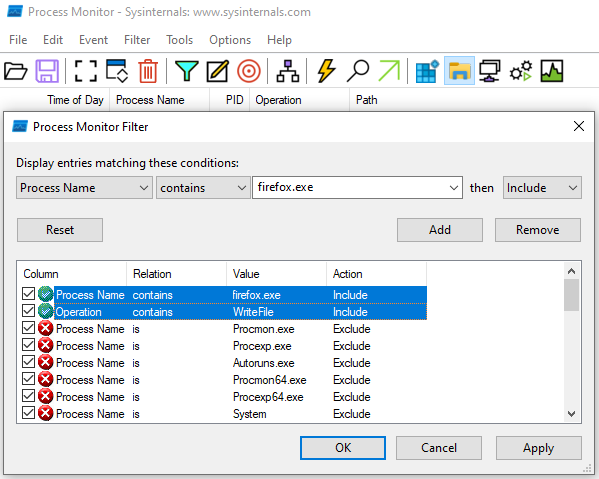
\includegraphics{bilder/process-monitor-filter.png}}
	%	\label{...}
		\caption{Tabelle mit wiederherstellbaren Dateien: Logfile 1 vs. Logfile 2}
	\end{figure}
	> Nur "File System Activity"
	> Process Name: contains "Browser-Prozess".exe
		- Firefox = firefox.exe
		- Tor = firefox.exe und tor.exe
		- Chrome = chrome.exe
		- Brave = brave.exe
	> Operation: contains "WriteFile"
- Gefiltertes Logfile als CSV exportieren, dann in Excel öffnen
- Irrelevante Spalten löschen: 
	> Time of Day
	> Process Name (Da in Process Monitor bereits nach Namen gefiltert wurde -> Alle Prozesse haben gleichen Namen)
	> Operation (Da in Process Monitor bereits nach Operation gefiltert wurde -> Alle Prozesse haben gleiche Operation „WriteFile“)
	> Result
	> Detail
- Gleiche Operationen (Duplikate) löschen
- Gruppieren nach browserspezifischen Speicherorten

Datenanalyse für jede geschriebene Datei:
I) Dateiextraktion
	1.	In Autopsy prüfen, ob Datei in Image von entsprechendem Snapshot vorhanden. Siehe Abbildung X: 
			> Logfile 1 -> Snapshot 2
			> Logfile 2 -> Snapshot 3
		Tor:
			> Logfile 1 -> Snapshot 2
			> Logfile 2-1 -> Snapshot 3-1
			> Logfile 2-2 -> Snapshot 3-2
	2.	Wenn ja, Dateien mit Autopsy extrahieren 
	3.	Wenn nein, prüfen, ob Datei in RAM gecacht:
		> Dazu Ausgabe von Volatiltiy Plugin "filescan" in entsprechendem RAM-Dump prüfen.
			> filescan: Das filescan-Plugin von Volatility durchsucht den Arbeitsspeicher nach Speicherbereichen, die Informationen über Dateien enthalten. Die Ausgabe des Plugins enthält eine Liste von Dateinamen, die im Speicher gefunden wurden. Können sein: Ausführbare Dateien, Bibliotheksdateien oder Konfigurationsdateien.
				% vol.py -f ram_dump.img windows.filescan > filescan.txt
		Welchen Dump bei welcher Logfile?
			> Logfile 1 -> RAM-Dump 2
			> Logfile 2 -> RAM-Dump 3
		Tor:
			> Logfile 1 -> RAM-Dump 2
			> Logfile 2-1 -> RAM-Dump 3-1
			> Logfile 2-2 -> RAM-Dump 3-2
		> Wenn Datei gefunden wurde: Datei mit dumpfiles und entsprechender virtueller Dateispeicheradresse extrahieren.
		\begin{figure}[h!]
			\centering
			\small
			\centerline{\resizebox{\linewidth}{!}{\input{bilder/volatility-filescan-dumpfiles-Latex.pdf_tex}}}
			\caption{Datensammlung Zeitpunkte Tor}
			\label{fig:jes}
		\end{figure}
	4. Wenn Datei auch nicht im RAM gecacht ist: Prüfen, ob es sich bei Datei um Hilfsdatei handelt. Dabei handelt es sich meistens um temporäre Dateien mit zusätzlicher Dateiendung (meistens .tmp)
	5. Wenn ja: Zur die Dateiendung der Hilfsdatei weglassen und bei Schritt 1 beginnen. z.B: Wenn Datei "some-file.json.tmp" nicht existiert, prüfen, ob Datei "some-file.json" existiert
	6. Wenn nein: Datei als "nicht wiederherstellbar" markieren
II) Dateianalsye (nachdem Datei extrahiert wurde)
	7. Datei mit entsprechdem Tool untersuchen 
	8. Wenn Datei nicht direkt untersuchbar ist: ggf. Mit zusätzlichem Tool Datei vorberarbeiten. z.B. Wenn es sich um komprimierte Dateien handelt
	9. In Excel-Tabelle markieren, ob Datei PB Artefakte enthält. Dabei gibt es drei Zustände: 
		- leere Datei
		- neuer (nicht-leerer) Inhalt
		- gleichbleibender Inhalt
	\begin{figure}[h!]
		\centering
		\small
		\centerline{\resizebox{\linewidth}{!}{\input{bilder/process_monitor_to_exce-Latexl.pdf_tex}}}
		\caption{TODO: Process Monitor Write Operation to Excel Spreadsheet}
		\label{fig:jes}
	\end{figure}

\subsubsection*{SQLite-Datenbänke}
- Besondere Rolle nehmen bei den ausgewählten Browsern SQLite Datenbänke ein.

"SQLite-Datenbanken sind besonders wichtig bei Webbrowsern wie Firefox, Tor, Chrome und Brave, da sie Informationen wie Lesezeichen, Browserverlauf, Caches, Cookies und Erweiterungsdaten speichern. Diese Datenbanken bieten Benutzern eine personalisierte Browsererfahrung und sind für Forensiker und Sicherheitsexperten von Bedeutung, um relevante Informationen über die Online-Aktivitäten eines Benutzers zu analysieren."

"Die Verwendung von SQLite-Datenbanken in diesen Webbrowsern bietet Effizienz, Flexibilität und eine einfache Möglichkeit, Daten zu organisieren und abzurufen. Für Forensiker und Sicherheitsexperten sind diese Datenbanken von Bedeutung, da sie wertvolle Informationen über die Online-Aktivitäten eines Benutzers enthalten können, die bei Untersuchungen, Sicherheitsanalysen oder forensischen Untersuchungen relevant sein können."

> Deshalb: Für jeden Browser werden die SQLite Datenbanken in allen Snapshots miteinander verglichen.
\begin{figure}[h!]
	\centering
	\small
	\centerline{\resizebox{\linewidth}{!}{\input{bilder/sqlite-methodology-Latex.pdf_tex}}}
	\caption{TODO: Process Monitor Write Operation to Excel Spreadsheet}
	\label{fig:jes}
\end{figure}
I) Dateiextraktion analog zu Dateien im Process Monitor
II) Dateianalyse:
	- SQLite Datenbank wird mit gleicher SQLite Datenbank aus vorherigem Snapshot verglichen (wenn vorhanden) -> Unterschiede in Excel-Tabelle festgehalten
	- Wichtig: Zu jeder SQLite Datenbank gibt es normalerweise eine .sqlite-wal Datei. 
		"Die Dateien mit der Erweiterung ".sqlite-wal" sind WAL-Dateien (Write-Ahead Log) in Verbindung mit SQLite-Datenbanken. Sie werden von SQLite verwendet, um Änderungen an einer Datenbank vorübergehend zu protokollieren, bevor sie dauerhaft in die Hauptdatenbankdatei geschrieben werden. Die WAL-Dateien dienen als Transaktions-Log und ermöglichen eine effiziente und sichere Aktualisierung der SQLite-Datenbanken, insbesondere in Situationen mit gleichzeitigen Schreibvorgängen."
		> Inhalte werden erst in WAL Datei geschrieben, dann in SQLite Datei
	- Deshalb: WAL Änderungen in SQLite Datei schreiben, danach sqldiff mit gleicher Datenbank ohne WAL Änderungen -> Unterschiede in Excel-Tabelle
		1) über sqlite3 Kommandozeile .sqlite Datenbank öffnen: % sqlite3 <Datenbank>.sqlite
		2) Über Pragma Befehl WAL Checkpoint durchführen: % sqlite3> PRAGMA wal_checkpoint;

\subsection{Uncommon Locations}

"Ungewöhnliche Speicherorte beziehen sich auf Verzeichnisse oder Orte, die nicht zu den gängigen oder standardmäßigen Speicherorten gehören."
= „Unbekannte Speicherorte“, nur durch tiefgehende forensische Analyse entdeckt
Blackbox-Analyse: \cite{Bonetti.2014} (Stringsuchen im gesamten Image mithilfe von Tool) 
= Durchsuchung des Beweismaterials ohne Vorwissen über Browserverhalten (d.h. welche Dateien geschrieben wurden) sowie ohne Vorverarbeitung der Dateien (z.B. Entpacken von Dateien).
Stattdessen: Untersuchen der Images nur mittels vordefinierter Funktionen von Forensik-Tools, da dies schnelles erstes Mittel von Forensikern, um nach Acquisition Phase Ergebnisse zu erhalten
- wichtigster Unterschied zu "Common Locations": Umgekehrte Suchrichtung => PB Artefakt (String) -> Alle Daten nach PB Artefakt durchsuchen
- Eigenschaften:
	> Wenn manuell durchgeführt, deutlich Zeitaufwändiger
	> Deshalb: Unterstützung durch Forensik-Tools. 
	> Vertrauen in die Vollständigkeit der Tools
- Beispiele in der Literatur:
	> “\$MFT”, “\$LogFile”, “Favicons”, “etilqs”, “Manifest.json”, “pagefile.sys.”, “unallocated space” and “slack space” \cite{Montasari.2015}	

Bei Browser Forensik hier oft verwendet: Stichwortsuchen über gesamtes Speicherabbild

Wichtig: String-Treffer muss Browser zugeordnet werden können
> Oft wiederkehrende Negativbeispiele in Literatur: gesamten RAM-Dump in Hexadezimaleditor geöffnet, danach: Stringsuche nach PB Artefakten. \cite{Rochmadi.2017, Md.2018, Montasari.2015}
> Problem: Gefundener String kein Indiz, dass tatsächlich Artefakt in Zusammenhang mit PB aufgetaucht ist.
> Gegenbeispiel: String in Textdatei in Desktop speichern. RAM Dump enthält String.

\subsubsection*{Analyse mit Autopsy}

Bei White-Box Analyse: Autopsy nur zur Dateiextraktion genutzt, hier: als konkretes forensisches Werkzeug

> Stichwortsuche über gesamtes Festplatten-Image
	*** TODO: Screenshot von Suchfunktion ***
> Zusätzlich: Autopsy PlugIns indexieren und kategoriesieren bereits Dateien
	- Web Bookmarks
	- Web Cookies
	- Web History
	- Web Categories

\subsubsection*{Analyse mit Volatility}

Bei White-Box Analyse: Volatility nur zur Dateiextraktion genutzt, hier: als konkretes forensisches Werkzeug

Wie oben ausführlich beschrieben: gefundener String im RAM muss Browser zugeordnet werden können -> Passendes Werkzeug = Volatility PlugIn "Yarascan". (siehe Kapitel Analysewerkzeuge)

*** TODO: konkrete Yara-Rules hier einfügen ***
> HTML-Fragmente: \cite{Said.2011} 
> Image als Hex: \cite{Ohana.2013}

> yarascan: Das Plugin "yarascan" ermöglicht die Durchführung einer YARA-basierten Malware-Erkennung im Arbeitsspeicherabbild. YARA ist eine flexible Regel-Engine, die verwendet werden kann, um nach bestimmten Mustern, Signaturen oder Verhaltensmerkmalen von Malware zu suchen. Das Plugin wendet YARA-Regeln auf den Arbeitsspeicher an und gibt potenzielle Treffer aus.
		% vol.py -f ram_dump.img windows.vadyarascan --yara-file yara_rules.yara > yarascan.txt
		Wichtig: yara\_rules.yara = In domainspecific Yara-Skriptsprache geschriebene Regeln, nach welchen RAM durchsucht wird.
		Hier: Einfache String-Pattern, die jeden Schritt des Browsing-Szenarios abdecken:
		*** TODO Beispielhafte Yara-Rules einfügen ***
		*** TODO: Erklärung Yara-Ausgaben, mit Screenshot ***
	=> Wichtig hier: Gibt PID des Prozesses und virtuelle Adresse des gefundenen Strings im Speicherbereich des Prozesses an

> Davon ausgehend: pslist: 
Das Plugin "pslist" wird verwendet, um eine Liste der aktiven Prozesse im Arbeitsspeicherabbild zu erstellen. Es extrahiert Informationen wie Prozessnamen, PID (Prozess-ID), Elternprozess, Startzeitpunkt, Priorität und andere Attribute für jeden laufenden Prozess.
		% vol.py -f ram_dump.img windows.pslist > pslist.txt
	=> Wichtig hier: Prozessname 	

> "String Kontext" herausfinden = Prüfen, ob in Speicherseite  über und unter gefundenen String weitere Zusammenhänge zu erkennen sind.
> Dazu: memmap: 
Das Plugin "memmap" dient dazu, eine detaillierte Karte des physischen Speichers des Systems zu erstellen. Es gibt Informationen über die physischen Speicherbereiche, deren Startadressen, Größen, Schutzattribute und andere relevante Details. Dieses Plugin kann bei der Analyse von Speicherlayout und -nutzung hilfreich sein.
		1) % vol.py -f ram_dump.img windows.memmap --pid <PID> > memmap.txt
			gibt Abbildung der Adressen des virtuellen Speichers auf die physikalische Adresse des Speicherbereichs des Prozesses mit der PID <PID>.
			Weiterhin und hier relevant: gibt Abbildung von virtuellen Adresse auf einen Datei-Offset an. Dieser bezieht sich auf die Datei, die erzeugt wird, wenn der Befehl mit dem --dump Flag ausgeführt wird:
		2) % vol.py -f ram_dump.img -o \dump_dir\ windows.memmap --pid <PID> --dump
			führt dies zur physischen Extraktion des Speicherbereichs des Prozesses mit der PID <PID> in eine separate Datei.		
 => Extrahierte Seite mit Hexeditor HxD untersuchen

\begin{figure}[h!]
	\centering
	\small
	\centerline{\resizebox{\linewidth}{!}{\input{bilder/yarascan_plugin_tree-Latex.pdf_tex}}}
	\caption{TODO: Process Monitor Write Operation to Excel Spreadsheet}
	\label{fig:jes}
\end{figure}


\subsection{Registry}
- zählt sowohl Common als auch Uncommon Location -> Deshalb eigene Kategorie
- Common: Analyse der Process Monitor Schreiboperationen in Registry
	Datenaufbereitung für jede Logfile:
	- Grundlage = Process Monitor Logfiles
	- Für Common Locations Filter setzen: 
		\begin{figure}[h!]
			\resizebox{\linewidth}{!}{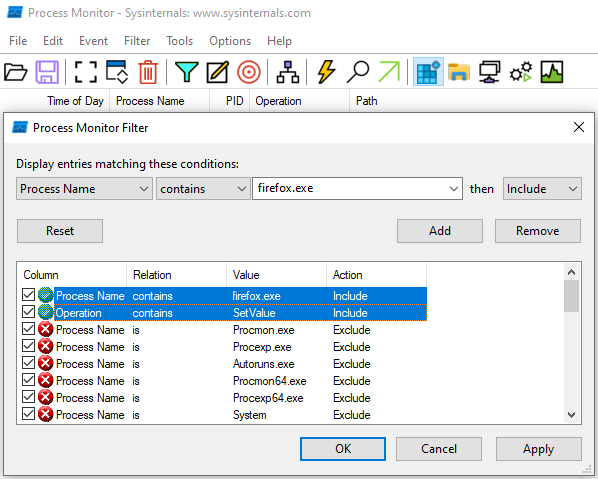
\includegraphics{bilder/process-monitor-filter-registry.png}}
		%	\label{...}
			\caption{Tabelle mit wiederherstellbaren Dateien: Logfile 1 vs. Logfile 2}
		\end{figure}	
		> Nur "Registry Activity"
		> Process Name: contains "Browser-Prozess".exe
			- Firefox = firefox.exe
			- Tor = firefox.exe und tor.exe
			- Chrome = chrome.exe
			- Brave = brave.exe
		> Operation: contains "SetValue"
	- Gefiltertes Logfile als CSV exportieren, dann in Excel öffnen
	- Gleiche Operationen (Duplikate) löschen
	- Browserspezifisches Gruppieren 
	Datenanalyse für jeden geschriebenen Registry Key: Value untersuchen (steht in CSV hinter jeder Key Schreiboperation)
	

- Uncommon: Stringsuche in bekannten Registry Hives mit Registry Explorer

	"Ein Registry Hive ist eine Datei in der Windows-Registry, die als Container für spezifische Arten von Konfigurations- und Nutzerdaten dient. Jedes Hive hat eine bestimmte Funktion, wie die Speicherung von Systemeinstellungen (System-Hives) oder individuellen Benutzerkonfigurationen (User-Hives). Die Hives im System32\\Config-Verzeichnis enthalten wichtige Informationen für das Betriebssystem, während die User-Hives unter dem jeweiligen Benutzerverzeichnis gespeichert werden. Diese Hives werden von Windows beim Start geladen und dienen als Quelle für Einstellungen und Informationen, die von verschiedenen Systemkomponenten und Anwendungen genutzt werden."	

	Quelle für Hives: % https://medium.com/@haircutfish/tryhackme-windows-forensics-1-task-3-accessing-registry-hives-offline-task-4-data-acquisition-b440f5be2a13
	
	System-Hives im Verzeichnis "% C:\Windows\System32\Config":
	===========================
    DEFAULT: Enthält die Standardkonfigurationseinstellungen für neue Benutzerprofile.
    SAM: Enthält die Sicherheitskontenverwaltungsdaten, einschließlich der Benutzerkonten und deren Kennwörter.
    SECURITY: Enthält Sicherheitsinformationen, die für die Zugriffssteuerung und Authentifizierung verwendet werden.
    SOFTWARE: Enthält Konfigurationsdaten für installierte Software und Anwendungen.
    SYSTEM: Enthält Systemkonfigurationseinstellungen und Gerätetreiberinformationen.

	User-Hives im Verzeichnis "% C:\Users<username>":
	=========================
    NTUSER.DAT: Enthält die individuellen Einstellungen und Konfigurationen für den angemeldeten Benutzer. 
    USRCLASS.DAT: Enthält Informationen über die Dateizuordnungen und Registrierungseinstellungen für den angemeldeten Benutzer im Zusammenhang mit seinen benutzerdefinierten Klassen. 

	Analyse der Hives für jeden VM-Snapshot: Alle Hives in eine Registry Explorer Sitzung, danach Stringsuche nach PB Artefakten	

